\paragraph{Methodology of the COORD subproject.}

%\begin{figure}
%\centering
%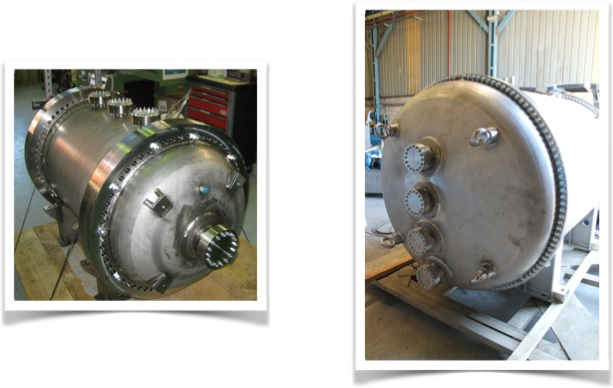
\includegraphics[height=8cm]{img/PV.jpg}
%\caption{The pressure vessel of NEW (left) and NEXT-100 (right).} \label{fig:PV}
%\end{figure}

%%%%%
\begin{figure}[t!b!]
\begin{center}
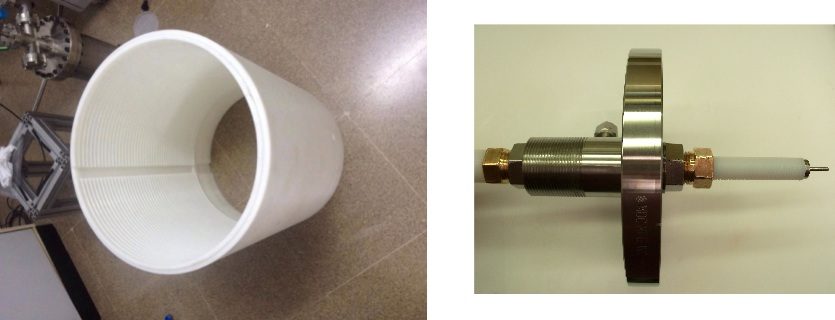
\includegraphics[width=.9\textwidth]{img/FC3.jpg}
\end{center}
\caption{\small Left: The NEW field cage body made of HDPE, fabricated in Spain; right: The anode HVFT manufactured in Texas.
} \label{fig:FC}
\end{figure}

%%%%%
\begin{figure}[t!b!]
\begin{center}
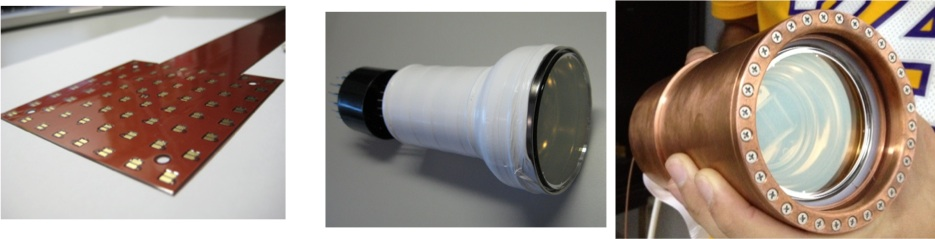
\includegraphics[width=.9\textwidth]{img/KDBandPMT.jpg}
\end{center}
\caption{\small Top left: the flexible Kapton Dice Board (KDB) circuit developed by NEXT for the tracking plane; mid: the R11410-10 PMT from Hamamatsu; bottom right: a PMT can prototype.} \label{fig:sensors}
\end{figure}

The first objective of the COORD subproject is the {\bf construction of the NEW detector}. The construction of NEW will involve:

\begin{enumerate}
\item {\em Construction of the NEW and NEXT-100 pressure vessels}.
The NEW and NEXT-100 pressure vessels were designed to withstand pressures in excess of 20 bar, and to operate with negligible losses at 15 bar. They are built using a 316Ti alloy of low activity. 
The design was a collaboration between IFIC and LBNL groups. They have been manufactured by several Spanish companies (TRINOS, MOVESA and ACYM). They will be shipped to LSC in Q1'15 and commissioned during Q2'15. 

\item {\em Construction of the NEW and NEXT-100 field cage (NFC)}
The NEW and NEXT-100 field cage produces an uniform electric ($\sim$ 300 V/cm) field inside the  detector that drifts the ionisation electrons to the anode, where they are further accelerated in the electric field produced between a pair of transparent grids, called the electroluminescent (EL) grids. 

The main body of the field cage is a high density polyethylene (HDPE) cylindrical shell with a 2.5\,cm wall thickness (Figure \ref{fig:FC}, left, shows the NEW field cage body).  The drift region consists of radiopure  copper strips connected with low radioactivity resistors.  The light tube consists of thin sheets of teflon, coated with tetraphenyl butadiene (TPB). The role of the TPB is to shift the UV light produced in xenon to the blue region (PMT and SiPMs operate best in this region, around 450 nm).  A high-voltage feedthrough (HVFT) in the cathode and another one in the anode, allow the definition of the voltages (Figure \ref{fig:FC}, right). The cathode HVFT is designed to withstand up to 100 kV, and the HVFT of the anode to withstand up to 40 kV. The design of the HVFT, identical for NEW and NEXT-100 improve those that were built for DEMO by the Texas A\&M group. The field cage and grids of NEW and NEXT-100 are also identical, to a scale 1:2. The grids use a stainless steel mesh with pitch 0.5 mm and wire diameter 30 microns, which results in an open area of 90\%. 

The construction of FC for NEW is currently under way (Q4' 2014). The HDPE body has been fabricated by the spanish company AIMPLAS. The HVFT and the grids have been manufactured at Texas. The  NFC will be tested at IFIC before shipping and installation in the LSC in Q1'15. The field cage will be commissioned in Q2'15. System commission, together with the rest of the systems will occur during Q3'15 and Q4'15.

\item {\em Construction of the NEW and NEXT-100 energy plane }
In NEW (NEXT-100) the energy measurement will be provided by the detection of EL light via PMTs, which will also record the scintillation light needed for $t_0$. Those PMTs will be located behind a transparent cathode.

A total of 12 (60) low-background, high-QE PMTs, model R11410-10 from Hamamatsu (Figure  \ref{fig:sensors}, mid panel) covering 32.5\% of the cathode will be deployed for NEW (NEXT-100) . The R11410-10 are large tubes, with a 3'' photocathode and low levels of  activity of the order of 1 mBq per unit in the Uranium and Thorium series. The PMTs are sealed into individual pressure resistant, vacuum tight copper enclosures (called PMT cans) coupled to 
sapphire windows, coated with ITO (for electrical conductivity) and TPB (Figure  \ref{fig:sensors}, right panel).

The NEW energy plane (NEP) is currently (Q4'15) under construction at IFIC. The ``PMT can'' design have been validated and production of the parts has started. The NEP will ship to LSC during Q1'15. It will be commissioned in Q2'15. System commission, together with the rest of the systems will occur during Q3'15 and Q4'15.

\item  {\em  Construction of the NEW and NEXT-100 tracking plane (NTP)}:
In NEW and NEXT-100 the tracking function is provided by a plane of multi-pixel photon counters (SiPMs) operating as a light-pixels and located behind the transparent EL grids. They are mounted in flexible radiopure Kapton Dice Boards (KDB). Each KDB hosts 64 SiPMs (Figure  \ref{fig:sensors}, left panel) .The NEW (NEXT-100) tracking plane will deploy 28 (112) such KDBs. 

The NTP is currently under construction at IFIC (Q4'14). The KDB production has been validated and prototypes have demonstrated excellent performance. The NTP will ship to LSC during Q1'15. It will be commissioned in Q2'15. System commission, together with the rest of the systems will occur during Q3'15 and Q4'15. 

\end{enumerate}
 
%%%%%%

The main objective of the COORD subproject is the {\bf fabrication of NEXT-100}. The construction will start in 2016 and will take 12 months. This fast schedule is possible thanks to several factors:
%
\begin{enumerate}
\item {\em Reuse of infrastructures}: the platform, pedestal, lead castle, gas system, clean tent, radon suppression system, online computing, slow controls and calibration hardware and procedures are common to NEW and NEXT-100 and will be extensively tested during NEW operation, thus ready for NEXT-100 phase.
\item {\em Early construction of pressure vessel}: The pressure vessel is a critical system, since it has to operate underground, at high pressure and with negligible losses. Designing, constructing and certifying it takes a long time. Luckily, this fact was understood at an early stage in the development of the project and the NEXT-100 pressure vessel (see Figure \ref{fig:PV}) was constructed during 2014, and has been tested and certified at the same time than the NEW pressure vessel. 
\item {\em Scalability of the field cage}: Some of the most delicate subsystems of the field cage (such as the HVFT) have been designed and tested to be operative in NEXT-100 (for example the HVFT in the cathode holds up to 100 kV voltage, while the nominal operation of NEXT-100 is 50 kV). The NEXT-100 field cage body will be constructed by the same company (AIMPLAS) that has built the NFC body, reusing the tools and procedures that have been put together for the task. This also applies to the construction of the EL grids. 
This makes possible to foresee an early assembly of the NEXT-100 field cage, in Q2'16, allowing for ample time for testing and debugging.

\item {\em Production chains for the energy and tracking planes}. The energy and tracking planes are composed of individual modules (PMT cans in the case of the energy plane, KDBs in the case of the tracking plane), mounted to supporting plates and connected to electronics. The structure of the systems is the same (as seen in Figure \ref{fig:EnergyPlane}). The number of modules (cans and KDBs) is larger in NEXT-100 (by about a factor 5), but, very importantly, the construction procedure is the same. This allow us to set {\em production chains}, PC, of both PMT cans and KDBs. The PCs will be extensively exercised during the construction of NEW, and are expected, therefore, to run smoothly during NEW construction.  

The production chains should be able to produce 20 PMT cans and 30 KDBs a month. We therefore, expect that the modules will be ready in Q1'16. Shipping and cleaning will take the best part of Q2'16. The systems should be assembled at the LSC in Q3'16, allowing for testing and debugging during Q4'16.
\end{enumerate}